\begin{activity} \label{A:1.2.3}
For the moving object whose position $s$ at time $t$ is given by the graph below, answer each of the following questions.  Assume that $s$ is measured in feet and $t$ is measured in seconds.
\begin{figure}[h]
\begin{center}
 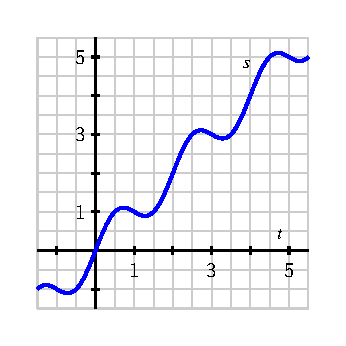
\includegraphics{figures/1_2_Act3.eps} \caption{Plot of the position function $y = s(t)$ in Activity~\ref{A:1.2.3}.}
\end{center}
\end{figure}
\ba
	\item Use the graph to estimate the average velocity of the object on each of the following intervals: $[0.5,1]$, $[1.5,2.5]$, $[0,5]$.  Draw each line whose slope represents the average velocity you seek.
	\item How could you use average velocities or slopes of lines to estimate the instantaneous velocity of the object at a fixed time?
	\item Use the graph to estimate the instantaneous velocity of the object when $t = 2$.  Should this instantaneous velocity at $t = 2$ be greater or less than the average velocity on $[1.5,2.5]$ that you computed in (a)?  Why?
\ea
\end{activity} 
\begin{smallhint}
\ba
	\item Remember that average velocity on an interval computes the quotient of ``change in $s$ over change in $t$.''  This is the slope of the line between the corresponding two points on the graph of $s$.
	\item Think about shorter and shorter time intervals and drawing the lines whose slopes represent average velocity.
	\item Think about zooming in on the graph at $t = 2$ and drawing a line that, up close, looks just like the curve $s(t)$.  What is the approximate slope of that line?
\ea
\end{smallhint}
\begin{bighint}
\ba
	\item Remember that average velocity on an interval computes the quotient of ``change in $s$ over change in $t$.''  This is the slope of the line between the corresponding two points on the graph of $s$.  For example, the average velocity on $[0.5,1]$ is $\frac{1-1}{1-0.5} = 0$.
	\item Think about shorter and shorter time intervals and drawing the lines whose slopes represent average velocity.  If those lines' slopes are approaching a single number, that number represents the instantaneous velocity.
	\item Think about zooming in on the graph at $t = 2$ and drawing a line that, up close, looks just like the curve $s(t)$.  What is the approximate slope of that line?  By drawing this line that looks like $s(t)$ near the point $(2,s(2))$ and comparing the line through the points $(1.5,s(1.5))$ and $(2.5, s(2.5))$, you should be able to compare the lines and see which has greater slope.
\ea
\end{bighint}
\begin{activitySolution}
\ba
	\item The average velocity on $[0.5,1]$ is the slope of the line joining the points $(0.5,s(0.5))$ and $(1,s(1))$, which is $AV_{[0.5,1]} = \frac{1-1}{1-0.5} = 0$.  On $[1.5,2.5]$, we similarly find $AV_{[1.5,2.5]} = \frac{3-1}{2.5-1.5} = 2$, and on $[0,5]$, we have $AV_{[0,5]} = \frac{5-0}{5-0} = 1$.
	\item  Take shorter and shorter time intervals and draw the lines whose slopes represent average velocity.  If those lines' slopes are approaching a single number, that number represents the instantaneous velocity.  For example, to estimate the instantaneous velocity at $t = 2$, we might consider average velocities on $[2,3]$, $[2,2.5]$, and $[2,2.25]$.
	\item  If we draw the line through $(2,2)$ and $(2.1,s(2.1))$, it looks like the line's slope is approximately 2.5: if we go over one grid-width, we appear to go up about 2.5.  The slope of this line is clearly greater than the slope of the line through $(1.5, s(1.5))$ and $(2.5, s(2.5))$, which is 2. Hence the instantaneous velocity at $t = 2$ is greater than the average velocity on $[1.5,2.5]$.
\ea
\end{activitySolution}
\aftera
